\subsection{Circular disk with an edge crack in tension}

\paragraph{}
Next, the present formulation is applied to problems with strong discontinuities and singularities.
The unique feature of the proposed framework is that the geometry is exactly represented by using NURBS and the singularities are captured semi-analytically without a priori knowledge of the asymptotic fields.
In the first example, consider a circular disk with an edge crack (see Fig.~\ref{iso_fig:circular_disk_geo_bc}) with Young’s modulus $E=\SI{1}{\newton \per \square \meter}$ and Poisson's ratio $\nu=0.3$.
    \begin{figure}[h!]
        \centering
        \scalebox{0.4}{
            \includegraphics{isogeometric_sbfem/images/circular_disk_geo_bc.eps}
        }
        \caption{Circular disk with an edge crack}
        \label{iso_fig:circular_disk_geo_bc}
    \end{figure}

The analytical displacements solution for mode \RN{1} are given by:
    \begin{subequations}
        \begin{align}
            u_x &= \frac{1}{2}\left[
                \left(
                    \kappa + \frac{n}{2} + (-1)^n
                \right) \cos \left(
                    \frac{n\theta}{2}
                \right) -
                \frac{n}{2} \cos \left(
                    \left(
                        \frac{n}{2} -2
                    \right) \theta
                \right)
            \right]\\
            u_y &= \frac{1}{2}\left[
                \left(
                    \kappa - \frac{n}{2} - (-1)^n
                \right) \sin \left(
                    \frac{n\theta}{2}
                \right) +
                \frac{n}{2} \sin \left(
                    \left(
                        \frac{n}{2} -2
                    \right) \theta
                \right)
            \right]\\
        \end{align}
    \end{subequations}

where $\kappa$ is the Kolosov constant defined in Eq.~\ref{iso_eq:kolosov_constant}.

The analytical stress solution for mode \RN{1} are given by:
    \begin{subequations}
        \begin{align}
            \sigma_{xx} &= \frac{n}{2}\left[
                \left(
                    2 + \frac{n}{2} + (-1)^n
                \right) \cos \left(
                    \left(
                        \frac{n}{2} - 1
                    \right)\theta
                \right) - \left(
                    \frac{n}{2} - 1
                \right)
                \cos \left(
                    \left(
                        \frac{n}{2} -3
                    \right) \theta
                \right)
            \right]\\
            \sigma_{yy} &= \frac{n}{2}\left[
                \left(
                    2 - \frac{n}{2} - (-1)^n
                \right) \cos \left(
                    \left(
                        \frac{n}{2} - 1
                    \right)\theta
                \right) + \left(
                    \frac{n}{2} - 1
                \right)
                \cos \left(
                    \left(
                        \frac{n}{2} -3
                    \right) \theta
                \right)
            \right]\\
            \tau_{xy} &= \frac{n}{2}\left[
                \left(
                    \frac{n}{2} - 1
                \right) \sin \left(
                    \left(
                        \frac{n}{2} - 3
                    \right)\theta
                \right) - \left(
                    \frac{n}{2} + (-1)^n
                \right)
                \sin \left(
                    \left(
                        \frac{n}{2} - 3
                    \right) \theta
                \right)
            \right]
        \end{align}
    \end{subequations}

\paragraph{}
In this example, the circular disk is represented by NURBS.
The control net and the location of control points are shown in Fig.~\ref{iso_fig:circular_disk_mesh} for different NURBS orders.
    \begin{figure}
        \begin{subfigure}[b]{0.5\linewidth}
            \centering
            \scalebox{0.4}{
                \includegraphics{isogeometric_sbfem/images/circular_disk_2nd_9cp.png}
            }
            \caption{9 control points, 2nd order}
        \end{subfigure}
        \begin{subfigure}[b]{0.5\linewidth}
            \centering
            \scalebox{0.4}{
                \includegraphics{isogeometric_sbfem/images/circular_disk_2nd_17cp.png}
            }
            \caption{9 control points, 2nd order}
        \end{subfigure}

        \begin{subfigure}[b]{0.5\linewidth}
            \centering
            \scalebox{0.4}{
                \includegraphics{isogeometric_sbfem/images/circular_disk_3rd_17cp.png}
            }
            \caption{9 control points, 2nd order}
        \end{subfigure}
        \begin{subfigure}[b]{0.5\linewidth}
            \centering
            \scalebox{0.4}{
                \includegraphics{isogeometric_sbfem/images/circular_disk_4th_17cp.png}
            }
            \caption{9 control points, 2nd order}
        \end{subfigure}
        \caption{Meshing of the circular disk with an edge notch}
        \label{iso_fig:circular_disk_mesh}
    \end{figure}

\paragraph{}
The circular disk is subjected to a far field tension and the displacement and the stress modes are computed by the proposed isogeometric SBFEM.
It is noted that only the boundary of the circular disk is discretized using the NURBS and no tensor product of the corresponding knot vectors is required to represent the unknown fields inside the domain.
The convergence of the numerical stress intensity factor (SIF) and the T-stress with mesh refinement is shown in Tab.~\ref{iso_tab:circular_disk_res}.

\begin{table}[]
\caption{T-stress and stress intensity factors for circular disk with an edge crack.}
\label{iso_tab:circular_disk_res}
\begin{tabularx}{\textwidth}{XXXXXXX}
\toprule
    Total    &   \multicolumn{2}{c}{NURBS $p=2$} &\multicolumn{2}{c}{NURBS $p=4$} &\multicolumn{2}{c}{NURBS $p=6$}\\
    \cmidrule{2-7}
    DOF      &   SIF     &   T-stress            &SIF     &   T-stress            &SIF     &   T-stress           \\
    \cmidrule{1-1} \cmidrule{2-3} \cmidrule{4-5} \cmidrule{6-7}
    18       &   2.3520  &   2.9442              &        &                       &        &                      \\
    34       &   2.8693  &   5.1991              &2.8838  &5.4050                 &        &                      \\
    74       &   2.8838  &   5.3112              &2.8840  &5.3445                 &2.8840  &5.3447                \\
    130      &   2.8840  &   5.3318              &2.8840  &5.3444                 &2.8840  &5.3444                \\
\bottomrule
\end{tabularx}
\end{table}

\paragraph{}
It can be seen that with mesh refinement the SIF and the T-stress converge.
Increasing the order of the NURBS functions increases the convergence behavior.
Eq.~\ref{iso_eq:isosbfem_fracture_stress_field} is the parametric equation for the stress field in the polar coordinates $r$ and $\theta$.
The terms $\left(
        r_\eta^{\lambda_i+1}(\eta)
        \boldsymbol{\psi}_{\sigma_i}(\eta)
    \right)$
in Eq.~\ref{iso_eq:isosbfem_fracture_stress_field} together with $\theta(\eta)$ in Eq.~\ref{lr_eq:sbfem_transform} are the stress modes describing the angular distribution at a constant radial coordinate $r$.
For the converged result, Fig.~\ref{iso_fig:circular_disk_modes} shows the displacement and the stress distribution at a constant radial coordinate r around the crack tip for mode \RN{1} fracture.
Each of the stress modes is normalized with its value of $\sigma_{yy}=0^\circ$ .
    \begin{figure}[h!]
        \begin{subfigure}[b]{1\linewidth}
            \centering
            \scalebox{0.4}{
                \includegraphics{isogeometric_sbfem/images/circular_disk_displacement_modes.png}
            }
            \caption{displacements}
        \end{subfigure}
        \begin{subfigure}[b]{1\linewidth}
            \centering
            \scalebox{0.4}{
                \includegraphics{isogeometric_sbfem/images/circular_disk_stress_modes.png}
            }
            \caption{stress}
        \end{subfigure}
    \caption{Displacement and stress modes of circular disk with an edge crack using cubic NURBS functions}
    \label{iso_fig:circular_disk_modes}
    \end{figure}

\paragraph{}
The stress modes from the scaled boundary formulation are compared with the analytical solutions and a very good agreement is observed in Tab.~\ref{iso_tab:circular_disk_res}.
The convergence of the displacement and stress modes with h and p refinement is shown in Fig.~\ref{iso_fig:circular_disk_convergence}.
It can be seen that with refinement the solution converges monotonically.
    \begin{figure}[h!]
        \begin{subfigure}[b]{1\linewidth}
            \centering
            \scalebox{0.65}{
                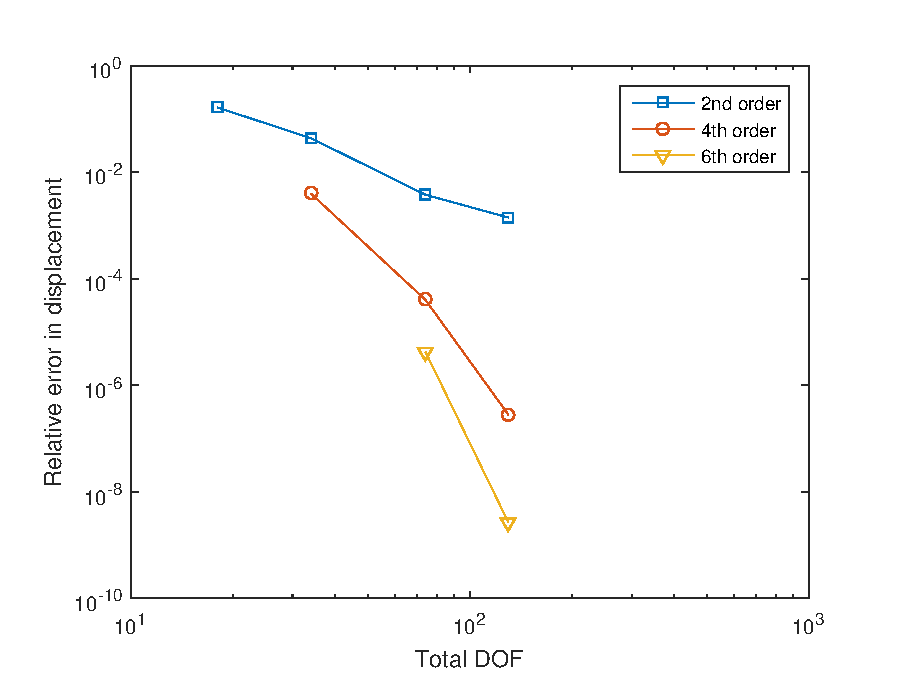
\includegraphics{isogeometric_sbfem/images/circular_disk_convergence_displacement.eps}
            }
            \caption{Displacement mode}
        \end{subfigure}

        \begin{subfigure}[b]{1\linewidth}
            \centering
            \scalebox{0.65}{
                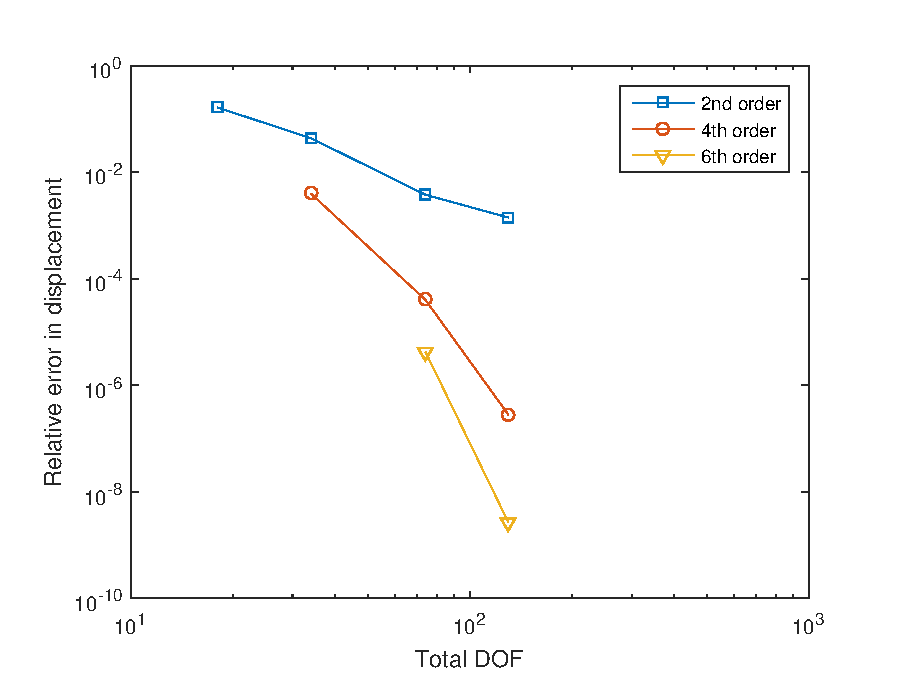
\includegraphics{isogeometric_sbfem/images/circular_disk_convergence_displacement.eps}
            }
            \caption{Displacement mode}
        \end{subfigure}
    \caption{Circular disk with an edge crack: convergence of the displacement mode and stress mode}
    \label{iso_fig:circular_disk_convergence}
    \end{figure}

